% Graphic for TeX using PGF
% Title: /home/ak/git/GM_Thesis/GM_Thesis_latex/GM_Thesis/img/distoptpair_example_detail.dia
% Creator: Dia v0.97.3
% CreationDate: Sat Apr 30 14:17:04 2016
% For: ak
% \usepackage{tikz}
% The following commands are not supported in PSTricks at present
% We define them conditionally, so when they are implemented,
% this pgf file will use them.
\ifx\du\undefined
  \newlength{\du}
\fi
\setlength{\du}{15\unitlength}
\begin{tikzpicture}
%\node[anchor=south west,inner sep=0] at (0,0) {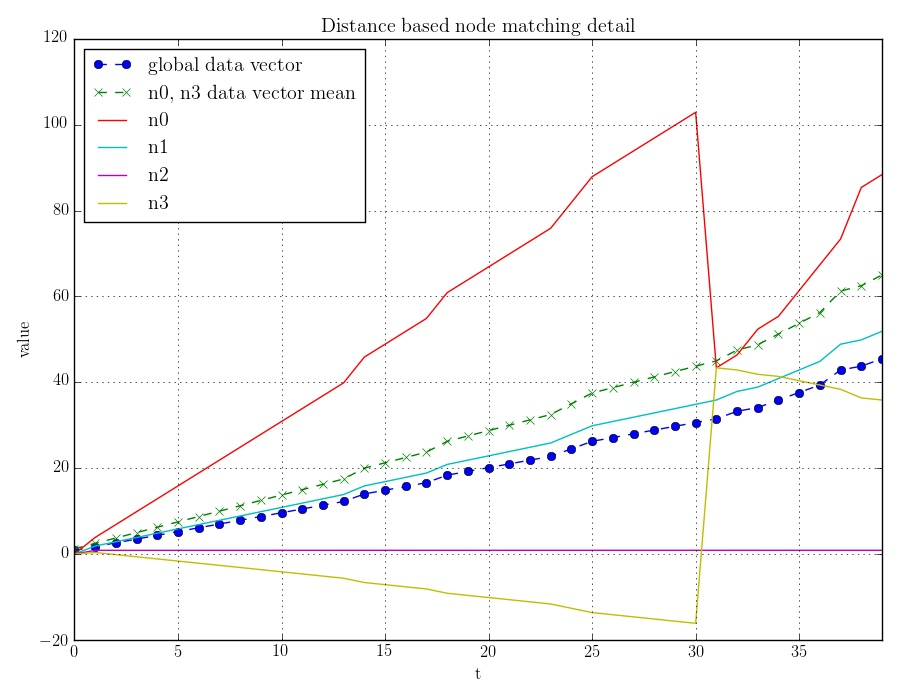
\includegraphics[width=\textwidth]{img/distoptpair_example_detail.jpeg}};
\node[anchor=south west,inner sep=0] (image) at (0,0) {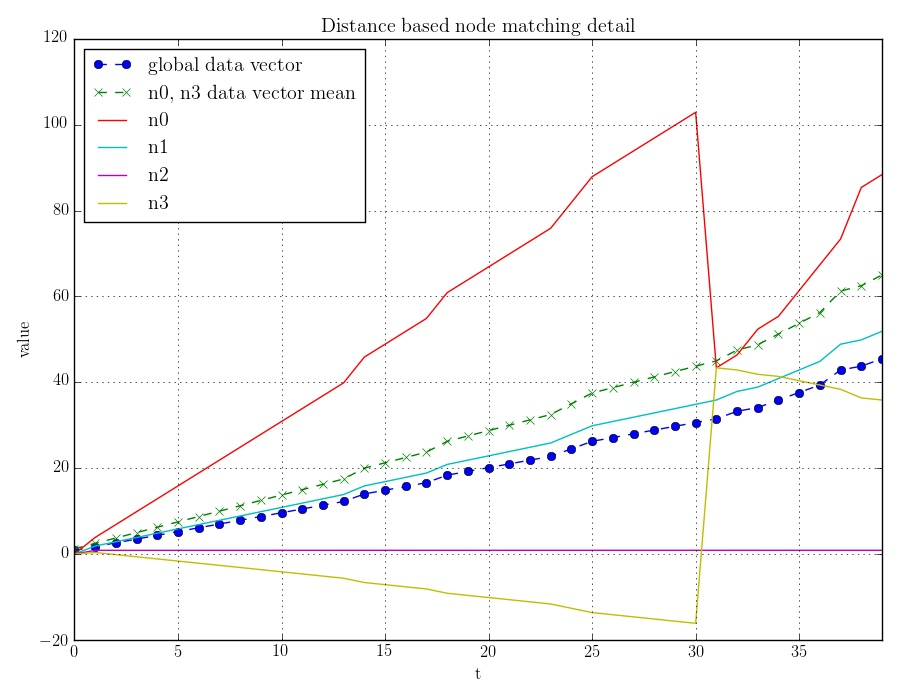
\includegraphics[width=0.9\textwidth]{img/distoptpair_example_detail.jpeg}};
\begin{scope}[x={(image.south east)},y={(image.north west)}]
\pgftransformxscale{1.000000}
\pgftransformyscale{-1.000000}
\definecolor{dialinecolor}{rgb}{0.000000, 0.000000, 0.000000}
\pgfsetstrokecolor{dialinecolor}
\definecolor{dialinecolor}{rgb}{1.000000, 1.000000, 1.000000}
\pgfsetfillcolor{dialinecolor}
% image rendering not supported\pgfsetlinewidth{0.150000\du}
\pgfsetdash{{1.000000\du}{1.000000\du}}{0\du}
\pgfsetdash{{0.300000\du}{0.300000\du}}{0\du}
\pgfsetbuttcap
{
\definecolor{dialinecolor}{rgb}{0.000000, 0.000000, 0.000000}
\pgfsetfillcolor{dialinecolor}
% was here!!!
}
\definecolor{dialinecolor}{rgb}{0.000000, 0.000000, 0.000000}
\pgfsetstrokecolor{dialinecolor}
\draw (29.025189\du,20.112478\du)--(29.040411\du,21.825022\du);
\pgfsetlinewidth{0.150000\du}
\pgfsetdash{}{0pt}
\pgfsetmiterjoin
\pgfsetbuttcap
\definecolor{dialinecolor}{rgb}{0.000000, 0.000000, 0.000000}
\pgfsetfillcolor{dialinecolor}
\fill (28.707812\du,19.565278\du)--(29.332788\du,19.559722\du)--(29.338343\du,20.184698\du)--(28.713368\du,20.190253\du)--cycle;
\definecolor{dialinecolor}{rgb}{0.000000, 0.000000, 0.000000}
\pgfsetstrokecolor{dialinecolor}
\draw (28.398102\du,19.880543\du)--(29.648053\du,19.869432\du);
\pgfsetlinewidth{0.150000\du}
\pgfsetdash{}{0pt}
\pgfsetmiterjoin
\pgfsetbuttcap
\definecolor{dialinecolor}{rgb}{0.000000, 0.000000, 0.000000}
\pgfsetfillcolor{dialinecolor}
\fill (29.357788\du,22.372222\du)--(28.732812\du,22.377778\du)--(28.727257\du,21.752802\du)--(29.352232\du,21.747247\du)--cycle;
\definecolor{dialinecolor}{rgb}{0.000000, 0.000000, 0.000000}
\pgfsetstrokecolor{dialinecolor}
\draw (29.667498\du,22.056957\du)--(28.417547\du,22.068068\du);
\pgfsetlinewidth{0.150000\du}
\pgfsetdash{{0.300000\du}{0.300000\du}}{0\du}
\pgfsetdash{{1.000000\du}{1.000000\du}}{0\du}
\pgfsetbuttcap
{
\definecolor{dialinecolor}{rgb}{0.000000, 0.000000, 0.000000}
\pgfsetfillcolor{dialinecolor}
% was here!!!
}
\definecolor{dialinecolor}{rgb}{0.000000, 0.000000, 0.000000}
\pgfsetstrokecolor{dialinecolor}
\draw (29.645300\du,9.050000\du)--(29.645300\du,30.275000\du);
\pgfsetlinewidth{0.150000\du}
\pgfsetdash{}{0pt}
\pgfsetmiterjoin
\pgfsetbuttcap
\definecolor{dialinecolor}{rgb}{0.000000, 0.000000, 0.000000}
\pgfsetfillcolor{dialinecolor}
\fill (29.332800\du,8.500000\du)--(29.957800\du,8.500000\du)--(29.957800\du,9.125000\du)--(29.332800\du,9.125000\du)--cycle;
\definecolor{dialinecolor}{rgb}{0.000000, 0.000000, 0.000000}
\pgfsetstrokecolor{dialinecolor}
\draw (29.020300\du,8.812500\du)--(30.270300\du,8.812500\du);
\pgfsetlinewidth{0.150000\du}
\pgfsetdash{}{0pt}
\pgfsetmiterjoin
\pgfsetbuttcap
\definecolor{dialinecolor}{rgb}{0.000000, 0.000000, 0.000000}
\pgfsetfillcolor{dialinecolor}
\fill (29.957800\du,30.825000\du)--(29.332800\du,30.825000\du)--(29.332800\du,30.200000\du)--(29.957800\du,30.200000\du)--cycle;
\definecolor{dialinecolor}{rgb}{0.000000, 0.000000, 0.000000}
\pgfsetstrokecolor{dialinecolor}
\draw (30.270300\du,30.512500\du)--(29.020300\du,30.512500\du);
% setfont left to latex
\definecolor{dialinecolor}{rgb}{0.000000, 0.000000, 0.000000}
\pgfsetstrokecolor{dialinecolor}
\node[anchor=west] at (26.345300\du,20.150000\du){($d_1$)};
% setfont left to latex
\definecolor{dialinecolor}{rgb}{0.000000, 0.000000, 0.000000}
\pgfsetstrokecolor{dialinecolor}
\node[anchor=west] at (30.510300\du,8.980000\du){($d_2$)};
\end{scope}
\end{tikzpicture}
